%
Equation \eqref{eq:r_condition} 
can be readily evaluated at any radial location in a model star generated with a 1D stellar structure and evolution program. However, predicting the efficiency of thermohaline mixing is much more challenging. A diffusive approximation is commonly taken for the turbulent mixing of chemicals such that the total mixing of chemical species is given by the sum of the molecular diffusivity and a turbulent mixing coefficient, $\Dth$. \textbf{This diffusion coefficient, $\Dth$, relates the rate of chemical mixing to the chemical composition gradient, and is broadly what is meant when referring to ``mixing efficiency" throughout this paper.} This quantity can be converted to the compositional Nusselt number discussed in the fluid dynamics literature, $\Numu$, using the formula

\begin{equation} \label{eq:Dth_from_Nu}
    \Dth = (\Numu - 1)\kappa_\mu.
\end{equation}

We call any model that predicts $\Dth$ as a function of stellar structure variables (e.g.~gradients and molecular diffusivities of chemicals and heat) a parameterized mixing model or mixing prescription. 
Efforts to develop thermohaline mixing prescriptions for use in models of stellar interiors date back many decades, see \citet{garaud_DDC_review_2018} for a full review. 
Such mixing prescriptions have been implemented in a variety of 1D stellar evolution programs \citep[see][and references therein]{lattanzio_etal_2015}, enabling studies of the effects of thermohaline mixing in stars across the Hertzprung-Russell diagram. 
Here, we briefly summarize the most commonly used and more recently developed prescriptions.

The \textit{de facto} thermohaline mixing model used in MESA (first described in \citealt{CantielloLanger2010} and implemented for public use in \citealt{mesa2}) is commonly referred to as the ``Kippenhahn model'' and was originally derived by \citet{Ulrich1972} and \citet{kippenhahn_etal_1980}.
Using arguments based on dimensional grounds and assumptions about the shapes and motions of discrete fluid parcels, they derived a mixing efficiency of the form

\begin{equation} \label{eq:Dth-kipp}
    \Dth = C_t \kappa_T R_0^{-1},
\end{equation}
\citep[see Eq.~(5) of][]{charbonnel_thermohaline_2007}
where $C_t$ is a free parameter, with plausible values ranging from $C_t = 658$ \citep{Ulrich1972} to $C_t = 12$ \citep{kippenhahn_etal_1980}. 
We note that Eq.~\eqref{eq:Dth-kipp} predicts finite mixing for $r \geq 1$ ($R_0 \geq 1/\tau$), even though thermohaline mixing is formally stabilized for these parameters.

Nevertheless, Eq.~\eqref{eq:Dth-kipp} is implemented in MESA as
\begin{equation} \label{eq:Dth-kipp-MESA}
    \Dth = \frac{3}{2} \alpha_{\rm{th}} \frac{K}{\rho C_P}R_0^{-1}
\end{equation}
\citep[see Eq.~(14) of][]{mesa2}. 
Here, $\alpha_{\rm{th}}$ is a dimensionless efficiency parameter related to $C_t$ by $C_t = 3\alpha_{\rm{th}}/2$, $K$ is the radiative conductivity, $\rho$ is the density, and $C_P$ is the specific heat at constant pressure, with $\kappa_T = K/(\rho C_P)$. 
The green curve in Fig.~\ref{fig:parameterization_compare} shows $\Dth/\kappa_\mu$ vs.~$r$ calculated according to Eq.~\eqref{eq:Dth-kipp-MESA} for $\tau = 10^{-6}$, which is a representative value for the thermohaline-unstable region of RGB stars, and the same $\alpha_{\rm{th}} = 2$ assumed in \citet{CantielloLanger2010}.

In addition to tension regarding the choice of \textbf{model parameters (e.g.~$\alpha_\mathrm{th}$) controlling overall mixing efficiency within a given 1D prescription} \citep[see e.g.][for further discussion]{Ulrich1972, kippenhahn_etal_1980, charbonnel_thermohaline_2007, CantielloLanger2010,traxler_etal_2011}, there have also been questions about the appropriate trends in \textbf{mixing efficiency} as a function of fluid parameters \textbf{(i.e.~how $\Dth$ should depend on quantities like $r$ and $\mathrm{Pr}$)} and therefore the stellar structure variables on which they depend \citep{garaud_DDC_review_2018}.
Thus, recent work has sought to refine these mixing prescriptions by performing numerical experiments with multi-dimensional simulations to more accurately parameterize mixing efficiency \citep{Denissenkov2010thermohaline,traxler_etal_2011}. 
\citet{traxler_etal_2011} and \citet{brown_etal_2013} performed 3D hydrodynamic simulations across a broad range of parameters. 
Not only did they find orders of magnitude less mixing than what is predicted by the Kippenhahn model with the \textbf{model} parameter required in \citet{charbonnel_thermohaline_2007} to find agreement with observations ($C_t = 1000$), they also developed new mixing prescriptions that fit their simulations much more closely. 
In the case of \citet{traxler_etal_2011}, the authors derived a mixing law by fitting an
analytic function 
of the form

\begin{equation} \label{eqn:trax_model}
   \Dth = \kappa_{\mu}\sqrt{\frac{\mathrm{Pr}}{\tau}}\left(a e^{-br}[1 - r]^c\right),
\end{equation}
to their simulation results,
where 

\begin{equation} \label{eq:Prandtl}
    \mathrm{Pr} = \frac{\nu}{\kappa_T}
\end{equation}
is the Prandtl number, with $\nu$ the kinematic viscosity,
%
and $a$, $b$, and $c$ are constants which they fit to data. 

While \citet{traxler_etal_2011} clearly showed their simulations are inconsistent with the mixing efficiency $\Dth$ implied by the Kippenhahn model with $\alpha_{\rm{th}}, C_t \sim 10^2-10^3$, it is important to note that their simulations generally explored $\mathrm{Pr}, \tau \sim 10^{-1}$, whereas these fluid parameters are generally of the order $10^{-6}$ in the radiative interiors of RGB stars. 
Thus, a fair question is whether mixing efficiency might increase to these larger values as $\mathrm{Pr}$ and $\tau$ approach $10^{-6}$. 
However, \citet{traxler_etal_2011} varied these parameters by an order of magnitude in their simulations, and investigated trends in $\Dth$. They found that mixing should not increase in this fashion, as indicated by the dependence of $\Dth$ on $\mathrm{Pr}$ and $\tau$ in Eq.~\eqref{eqn:trax_model}, which makes an argument that these models can be made to fit the observational data difficult to justify. 

\citet{brown_etal_2013} note that the model in Eq.~\eqref{eqn:trax_model} performs well at high $R_0$, but underestimates mixing at low $R_0$, particularly in the stellar regime of low Pr and $\tau$.
They develop a semi-analytical model for thermohaline mixing,

\begin{equation}
    \Dth = \kappa_{\mu}C^2\frac{\lambda^2}{\tau l^2(\lambda + \tau l^2)},
    \label{eqn:brown_model}
\end{equation}
where $\lambda$ is the growth rate of the fastest-growing linearly unstable mode, $l$ is its horizontal wavenumber, and $C \approx 7$ was fit to data from 3D hydrodynamic simulations.
Both $\lambda$ and $l$ are functions of $\mathrm{Pr}$, $\tau$, and $R_0$, and are obtained by finding the roots of a cubic and quadratic polynomial (their Eqs.~19 and 20).
The orange curve in Fig.~\ref{fig:parameterization_compare} shows $\Dth/\kappa_\mu$ vs.~$r$ calculated according to Eq.~\eqref{eqn:brown_model} for $\mathrm{Pr} = \tau = 10^{-6}$, representative values for the thermohaline-unstable regions of RGB stars. 
Note that $\Dth/\kappa_\mu \to 0$ as $r \to 1$ as expected, since the thermohaline instability becomes stable for $r \geq 1$.
We see that Eq.~\eqref{eq:Dth-kipp-MESA} with $\alpha_{\rm{th}} = 2$ agrees with this prescription for some values of $r$, suggesting that significantly larger values of $\alpha_{\rm{th}}$ are not consistent with 3D hydrodynamic simulations. 
While the general dependence of $\Dth/\kappa_\mu$ on $r$ is significantly different between these two models, they do both feature monotonically decreasing values of $\Dth/\kappa_\mu$ versus $r$. 
This prescription is implemented in MESA and has since been used in \citet{bauer_bildsten_2019} and other works. 

\citet{harrington} extended the work of \citet{brown_etal_2013} by performing 3D magnetohydrodynamic (MHD) simulations of thermohaline mixing with initially uniform, vertical magnetic fields of various strengths to approximate the effects of magnetic fields from external processes including, for instance, a global dipole field or a large-scale magnetic field left behind by a dynamo acting in the receding convective envelope. 
They found that magnetism strictly increases mixing efficiency, sometimes dramatically.
They developed a mixing prescription that accounts for this effect by building on the model of \citet{brown_etal_2013}.
The strength of the magnetic field is introduced into their model through their parameter $H_B$, which is proportional to the square of the magnetic field strength and depends on other stellar structure variables \citep[see Eq.~19 of][]{harrington}.
Their mixing prescription is of the form

\begin{equation} \label{eq:harrington_model}
    \Dth = \kappa_{\mu}K_B\frac{w_f^2}{\tau (\lambda + \tau l^2)},
\end{equation}
where $w_f$ is obtained by solving a quartic polynomial that includes the magnetic field strength through $H_B$, and $K_B \simeq 1.24$ is directly related to the constant $C$ in Eq.~\eqref{eqn:brown_model}.

This mixing prescription agreed remarkably well with their 3D simulations, which were limited to $r = 0.05$ but ranged in magnetic field strength over several orders of magnitude.
The prescription, which has not yet been implemented in MESA at the time of this writing, has two asymptotic limits, one where $\hat{w}_f^2 \propto B_0^2$ when the magnetic field strength $B_0$ is large, and one which reduces to the model of \citet{brown_etal_2013} when $B_0$ is small.

The purple curve in Fig.~\ref{fig:parameterization_compare} shows $\Dth/\kappa_\mu$ vs.~$r$ calculated according to Eq.~\eqref{eq:harrington_model} for the same parameter choices as the orange curve, and with $H_B = 10^{-6}$, appropriate for the thermohaline zone of a 1.1 $M_\odot$ star at [Fe/H] = -0.2 and a magnetic field whose strength is $\mathcal{O}(100 \,\mathrm{G})$. 
Note that this magnetic field strength dramatically increases mixing efficiency relative to the hydrodynamic values, particularly at larger values of $r$, whereas the model predicts the same mixing as the Brown model for $r \lesssim 10^{-5}$. 
For larger values of $r$, the dependence of $\Dth/\kappa_\mu$ on $r$ is profoundly different than either of the hydrodynamic models, with $\Dth/\kappa_\mu$ increasing with $r$, even as the thermohaline instability approaches marginal stability as $r \to 1$.

\textbf{The dramatic enhancement in mixing efficiency predicted by this model for magnetic field strengths of even $\mathcal{O}(100\,\mathrm{G})$ presents a promising resolution to the tension discussed above, namely that 1D stellar evolution models can only reproduce observations by assuming that mixing is far more efficient than what is seen in 3D hydrodynamic simulations. 
%the mixing efficiency needed in 1D stellar evolution models in order to agree with observations is much larger than what is consistent with 3D hydrodynamic simulations. 
However, while their prescription may predict mixing efficiencies that are comparable in overall magnitude to that of the Kippenhahn model with $C_t \sim 10^3$, the two prescriptions yield qualitatively different trends in $\Dth$ vs $r$.} 
Given the variance of the predictions of these models, we focus in this paper on showing how observations can be used to suggest the \textit{trends} in mixing that models should hope to explain rather than on trying to calibrate \textbf{model parameters controlling} the overall mixing \textit{efficiency} for a particular model, as has been done before, in order to provide a framework in which we can distinguish between mixing prescriptions.

%are not.

\begin{figure}
    \centering
    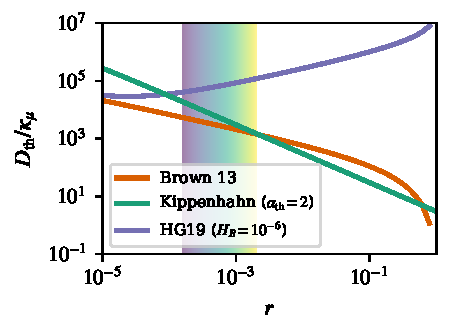
\includegraphics[width=\columnwidth]{Nu_models_comparison.pdf}
    \caption{ 
    Prescriptions of the compositional diffusivity due to thermohaline mixing $D_{\rm th}$ normalized by the molecular diffusivity $\kappa_{\mu}$ are plotted against the reduced density ratio $r$. For each prescription, we use $\mathrm{Pr} = \tau = 10^{-6}$, consistent with the conditions in these regions of RGB stars.
    We plot two hydrodynamic models, the \citet{brown_etal_2013} model (orange) and the \citet{kippenhahn_etal_1980} model with $\alpha_{\rm th} = 2$ (green). In both cases, the mixing efficiency decreases with $r$.
    The \citet{harrington} model (HG19) is also shown; it includes magnetic fields, which cause mixing efficiency to increase with $r$ for these parameters.
    The plotted curve for the HG19 model depends on $H_B$, which depends on the stellar structure and magnetic field strength; the plotted value is characteristic of the structure in the thermohaline zone of a 1.1 $M_\odot$ star at [Fe/H] = -0.2 with a magnetic field whose strength is $\mathcal{O}(100 \,\mathrm{G})$.
    The purple-to-yellow color gradient plotted in the background denotes the range of $r$ values that we measure in our grid of 1D stellar evolution models, which are displayed in Fig.~\ref{fig:mesa_r_spread}.
    }
    \label{fig:parameterization_compare}
\end{figure}
